% -*- root: ../main.tex -*-
%!TEX root = ../main.tex
% this file is called up by main.tex
% content in this file will be fed into the main document
% vim:textwidth=80 fo=cqt

In this  section, the performance  of the  basic \gls{spm} is  discussed through
desktop  simulation and  by comparison  against a  standard \gls{dfn}  benchmark
model incorporating the full \gls{p2d} dynamics.

\subsection{Cell Parametrisation}\label{subsec:spmp2dparametrisation}
% -*- root: ../main.tex -*-
%!TEX root = ../main.tex
% this file is called up by main.tex
% content in this file will be fed into the main document
% vim:nospell

\begin{table}[!htbp]
    \small
    \caption[Simulation parameters of  an \protect{\gls{lco}} cell]{Complete set
        of  parameters for  simulating the  \protect{\gls{p2d}} and  \protect{\gls{spm}}
        implementations  of an  \protect{\gls{lco}} cell  (with \ch{LiCoO_2}--\ch{LiC_6}
        electrode   pair  and   \ch{LiPF_6}   electrolyte).   The  highlighted   entries
        represent the  parameters exclusive  to \gls{p2d} model.\quad  \protect{$j \in
    \{\text{pos},\text{sep},\text{neg}\}$}}
    \label{tbl:lcoSimParamsSPMp2d}
    \vspace{-2.6229525pt}
    \begin{threeparttable}
        \centering
        \begin{varwidth}[t]{0.48\linewidth}
            \begin{tabular*}{\textwidth}{@{} l @{\extracolsep{\fill}} r @{}}
                \multicolumn{2}{c}{\textbf{System Conditions}} \\
                \toprule
                \multicolumn{1}{@{}l}{Parameter} \\
                \midrule

                Lower cutoff cell voltage, $V_\text{min}$ (\si{\volt}) & \tnote{a}2.50   \\
                Upper cutoff cell voltage, $V_\text{max}$ (\si{\volt}) & \tnote{b}4.30   \\
                Cell temperature, $T_\text{cell}$ (\si{\kelvin})       & \tnote{c}298.15 \\

                \bottomrule
            \end{tabular*}
        \end{varwidth}
        \hfill
        \begin{varwidth}[t]{0.48\linewidth}
            \begin{tabular*}{\textwidth}{@{} l @{\extracolsep{\fill}} r @{}}
                \multicolumn{2}{c}{\textbf{Other Constants}} \\
                \toprule
                \multicolumn{1}{@{}l}{Parameter} \\
                \midrule

                Faraday constant, $F$ (\si{\coulomb\per\meter})                                                        & 96487         \\
                Universal gas constant, $R$ (\si{\joule\per\mole\per\kelvin})                                          & 8.314         \\
                \textcolor{imperialblue}{\emph{Init.}}\ electrolyte conc., $c_\text{e,0}$ (\si{\mole\per\meter\cubed}) & \tnote{c}1000 \\

                \bottomrule
            \end{tabular*}
        \end{varwidth}

        \bigskip
        \vspace{-2.6229525pt}
        % \vfill

        \begin{tabular*}{\textwidth}{@{} =P{7.5cm} @{\extracolsep{\fill}} +l +c +r @{}}
            \multicolumn{4}{c}{\textbf{Thermodynamic, Kinetic, Geometric and Transport Parameters}} \\
            \toprule
            \multicolumn{1}{@{}l}{Parameter} & \multicolumn{1}{l}{Pos} & \multicolumn{1}{c}{Sep} & \multicolumn{1}{r@{}}{Neg}\\
            \midrule

            \rowstyle{\color{imperialblue}} Bruggeman coefficient, $\text{brugg}_j$                                                 & \tnote{c}\num{4}        & \tnote{c}\num{4}                               & \tnote{c}\num{4}        \\
            \rowstyle{\color{imperialblue}} Intrinsic electrolyte diffusivity, $D$ (\si{\meter\squared\per\second})               & \tnote{d}\num{3.22e-10} & \tnote{d}\num{3.22e-10}                        & \tnote{d}\num{3.22e-10} \\
            \rowstyle{\color{imperialblue}} Intrinsic electrolyte conductivity, $\kappa$ (\si{\siemens\per\meter})                &
            \multicolumn{3}{c}{\textcolor{imperialblue}{\Vhrulefill{} see table note \emph{e} \&~\cref{subsec:basicspmsimsetup} \Vhrulefill{}}}\\
            \rowstyle{\color{imperialblue}} \ch{Li^+} transference number, $t^0_\text{+}$                                           & \tnote{c}\num{0.363}    & \tnote{c}\num{0.363}                           & \tnote{c}\num{0.363}    \\
            \rowstyle{\color{imperialblue}} Intrinsic electronic conductivity, $\sigma_j$ (\si{\siemens\per\meter})                 & \tnote{c}\num{100.00}   & ---                                            & \tnote{c}\num{100.00}   \\
            Thickness, $l_j$ (\si{\meter})                                                          & \tnote{c}\num{88e-6}    & \textcolor{imperialblue}{\tnote{c}\num{25e-6}} & \tnote{f}\num{72e-6}    \\
            Electrolyte porosity, ${\varepsilon}_j$                                                 & \tnote{c}\num{0.385}    & \tnote{c}\num{0.724}                           & \tnote{c}\num{0.485}    \\
            Filler vol.\ fraction, ${\varepsilon}_{\text{fi}_j}$                                    & \tnote{c}\num{0.025}    & ---                                            & \tnote{c}\num{0.033}    \\
            Particle radius, $R_\pj$ (\si{\meter})                                                  & \tnote{c}\num{2e-6}     & ---                                            & \tnote{c}\num{2e-6}     \\
            Specific interfacial surface area, $a_\sj$ (\si{\meter\squared\per\meter\cubed})        & \tnote{g}\num{885e3}    & ---                                            & \tnote{g}\num{723.6e3}  \\
            Electrode diffusivity, $D_{\text{s}_j}$ (\si{\meter\squared\per\second})                & \tnote{c}\num{1e-14}    & ---                                            & \tnote{c}\num{3.9e-14}  \\
            Stoichiometry, 0\% SOC, ${\theta}_{\text{min}_j}$                                       & \tnote{h}\num{0.9917}   & ---                                            & \tnote{h}\num{0.0143}   \\
            Stoichiometry, 100\% SOC, ${\theta}_{\text{max}_j}$                                     & \tnote{c}\num{0.4955}   & ---                                            & \tnote{c}\num{0.8551}   \\
            Max concentration, ${c_\text{s,max}}_j$ (\si{\mole\per\meter\cubed})                    & \tnote{c}\num{51554}    & ---                                            & \tnote{c}\num{30555}    \\
            Reaction rate coefficient, $k_\jr$ (\si{\meter\tothe{2.5}\mole\tothe{-0.5}\per\second}) & \tnote{c}\num{2.33e-11} & ---                                            & \tnote{c}\num{5.03e-11} \\
            Overall active surface area, $A$ (\si{\meter\squared})                                  & \tnote{i}\num{2.053}    & ---                                            & \tnote{i}\num{2.053}    \\
            Open circuit potential, $U_j$ (\si{\volt})                                              & \tnote{k}see table note & ---                                            & \tnote{m}see table note \\
            \bottomrule
        \end{tabular*}

        \bigskip
        \vspace{-2.6229525pt}
        % \vfill
        %%%%%%%%%%%%%%%%%%%%%%%%%%%% SIMULATION PARAMS TABLE %%%%%%%%%%%%%%%%%%%%%%%%%%%%%
        \begin{tabular*}{\textwidth}{@{} =P{7.5cm}  +l@{\extracolsep{\fill}}+c +r @{}}
            \multicolumn{4}{c}{\textbf{Spatial Discretisation}} \\
            \toprule
            \multicolumn{1}{@{}l}{Parameter} & \multicolumn{1}{l}{Pos} & \multicolumn{1}{c}{Sep} & \multicolumn{1}{r@{}}{Neg}\\
            \midrule

            \rowstyle{\color{imperialblue}} Nodes, through-thickness (axial), $N_{\text{a}_j}$          & \num{15} & \num{15} & \num{15} \\
            \rowstyle{\color{imperialblue}} Nodes, within spherical particle (radial), $N_{\text{r}_j}$ & \num{10} & ---      & \num{10} \\

            \bottomrule
        \end{tabular*}

        \medskip
        \vspace{-2.6229525pt}
        % \vfill
        \begin{tablenotes}[para,flushleft]
            \begin{scriptsize}
            \item[a] Ref.~\cite{Northrop2011}
            \item[b] Set to $\approx $\SI{100}{\milli\volt} above the cell's \gls{ocp} at \SI{100}{\percent} cell \gls{soc}
            \item[c] Ref.~\cite{Subramanian2009}
            \item[d] Computed at $T_\text{cell} = \SI{298.15}{\kelvin}$ using coefficients from table \rom{2} in Ref.~\cite{Valoen2005}\\%\fxnote{cross-ref to actual equation}
            \item[e] Computed at $T_\text{cell} = \SI{298.15}{\kelvin}$ using coefficients from table \rom{3} in Ref.~\cite{Valoen2005} at $c_\text{e,0}= \SI{1000}{\mole\per\meter\cubed}$\\
            \item[f] Set up for capacity balance of electrodes such that $l_\text{neg} = 1.22 \times l_\text{pos}$ here.
            \item[g] Computed as per~\cref{eq:specificsurfarea}\\
            \item[h] Obtained as residual stoichiometries after a C/\num{500} simulated discharge from \SI{100}{\percent} cell \gls{soc} to \SI{2.7}{V}
            \item[i] Chosen so that current density for the electrochemical layer is \SI{29.23}{\ampere\per\meter\squared} for \SI{60}{\ampere} applied current
            \end{scriptsize}
            \vspace{1ex}
            \item[k] $ \mathcal{U(\theta_\text{pos})} = \textstyle \frac{-4.656 + 88.669\theta_\text{pos}^2 - 401.119\theta_\text{pos}^4 + 342.909\theta_\text{pos}^6 - 462.471\theta_\text{pos}^8 + 433.434\theta_\text{pos}^{10}}{-1 + 18.933\theta_\text{pos}^2 - 79.532\theta_\text{pos}^4 + 37.311\theta_\text{pos}^6 - 73.083\theta_\text{pos}^8 + 95.96\theta_\text{pos}^{10}}$ \\[0.25em]
            \begin{footnotesize}
            \item[m] $\mathcal{U(\theta_\text{neg})} = 0.7222 + 0.1387\theta_\text{neg} + 0.029\theta_\text{neg}^{0.5} - \frac{0.0172}{\theta_\text{neg}} + \frac{0.0019}{\theta_\text{neg}^{1.5}} + 0.2808 e^{(0.9 - 15\theta_\text{neg})} - 0.7984 e^{(0.4465\theta_\text{neg} - 0.4108)}$\vfill
            \end{footnotesize}
        \end{tablenotes}
    \end{threeparttable}
\end{table}

% Electrolyte diffusivity, $D_j$ \si{(m^2.s^{-1})}                         & \multicolumn{3}{c} {\Vhrulefill{} refer to equation in \tnote{g} \Vhrulefill{}} \\
% \item[g] $ D_j = 10^{-4} \times 10^{-4.43 - \frac{54}{T_\text{cell} - 229 - 5\times10^{-3} c_\text{e}(x,t)} - 0.22\times10^{-3} c_\text{e}(x,t)}, \quad \jinpossepneg $\\

% $\scriptstyle 10^{-4} c_\text{e} \left(-10.5 + \num{0.668e-3} c_\text{e} + \num{0.494e-6} c_\text{e}^2 + (0.074 - \num{1.78e-5}) c_\text{e} - \num{8.86e-10} c_\text{e}^2\right)T_\text{cell} + \left(\num{-6.96e-5} + \num{2.8e-8} c_\text{e})T_\text{cell}^2\right)^2$
% \tnote{e}\num{26.24e-3} & \tnote{e}\num{328.15e-3}                       & \tnote{e}\num{66.08e-3} \\


\Cref{tbl:lcoSimParamsSPMp2d} lists  the simulation  parameters of  an \gls{lco}
cell  whose positive  and negative  electrodes are  \ch{LiCoO_2} and  \ch{LiC_6}
respectively.  The  electrolyte in  this  system  consists of  \ch{LiPF_6}  salt
in  a   solution  of   \gls{ec}/\gls{dmc}/\gls{emc}  in   a  1:1:1   ratio.  The
standard  set  of  \gls{dfn}  parameters have  been  extensively  described  and
documented  in  literature.  The   detailed  characterisation  of  the  physical
properties  of  lithium-ion  cells  falls  outside the  scope  of  this  thesis.
Here, the  vast majority  of electrochemical  parameters, \viz{}  the geometric,
thermodynamic, kinetic  and transport properties  of the cell have  been sourced
from  Subramanian~\etal{}~\cite{Subramanian2009}.   The  significance   of  each
of  the  parameters  in  the  context of  the  modelling  assumptions  discussed
in~\cref{subsec:basicspmassumptions} is examined.


The simulation parameters that are applicable exclusively to the \gls{p2d} model
are shown as  highlighted text in~\cref{tbl:lcoSimParamsSPMp2d}. It  can be seen
that only a  subset of the isothermal \gls{dfn} model's  parameters are required
for the the \gls{spm}. In particular, there is no requirement to estimate any of
the electrolyte-related  parameters in  each electrode region.  Furthermore, the
properties of the separator material which  are necessary in the \gls{dfn} model
are also  not considered in the  \gls{spm} computations. A brief  enumeration of
the additional  \gls{p2d}-specific parameters in the  context of parametrisation
requirements is provided here.

\begin{enumdescriptnum}[leftmargin=!,itemsep=1ex,labelwidth=\widthof{$\symbf{\text{brugg}_j}\ \scriptstyle (\times 3)$abc}
    ,partopsep=0pt
    ,topsep=0pt
    ]

    \customenum{\text{brugg}_j}{3}  The  empirical Bruggeman  coefficient  helps
    to   define   the  effective   values   of   conductivity  and   diffusivity
    of   the  electrolyte.   Although  an   identical   value  of   4  is   used
    in~\cref{tbl:lcoSimParamsSPMp2d}, in  principle all  three regions  can have
    different values of brugg and need to be parametrised separately.

    \customenum{D}{1}  The  intrinsic  electrolyte   diffusivity  of  a  typical
    electrolyte  consisting  of  \ch{LiPF_6}  salt in  an  organic  solvent  was
    experimentally  characterised   and  provided  as  a   table  of  polynomial
    coefficients  by  Valøen  and  Reimers~\cite{Valoen2005}.  Evaluating  this
    polynomial  at a  cell  temperature of  \SI{298.15}{\kelvin}  results in  an
    intrinsic diffusivity of \SI{3.22e-10}{\meter\squared\per\second}. Since the
    intrinsic  diffusivity is  a material  property  and is  independent of  the
    region within the cell, it needs to be parametrised only once.

    \customenum{\scalebox{1.35}{$\kappa$}}{1}   Like    the   diffusivity,   the
    intrinsic electrolyte conductivity is also a material property and its value
    is independent  of the region within  the cell. Unlike the  diffusivity, the
    electrolyte conductivity  is a strong  function of its  ionic concentration.
    Thus, the polynomial proposed by Valøen and Reimers~\cite{Valoen2005} needs
    to  be evaluated  at  $T_\text{cell}= \SI{298.15}{\kelvin}$  and  has to  be
    updated during the  simulation as salt concentration  within the electrolyte
    changes over time. A discussion on the choice of initial concentration is
    provided in~\cref{subsec:basicspmsimsetup}.

    \customenum{\scalebox{1.25}{$t$}_+^0}{1}  The  cationic transference  number
    measures the relative  mobility of the \ch{Li^+} ion in  the organic solvent
    and is  independent of  the region  within the  cell. Hence,  this intrinsic
    property is to be parametrised only once (per solvent).

    \customenum{\scalebox{1.25}{$\sigma$}_j}{2} The intrinsic conductivity of the solid
    phase depends on the material used in the porous electrodes. Although a
    simplified assumption of equal conductivity is used for the two electrodes,
    in practice, this property needs to be characterised for each of the two
    electrodes.

\end{enumdescriptnum}

\sisetup{detect-weight=true}   Thus,   neglecting   Arrhenius-type   temperature
dependence of  physical properties and their  corresponding activation energies,
the basic  \gls{spm} facilitates the  ability to afford  physics-based modelling
capabilities with  \emph{eight} fewer parameters than  the equivalent isothermal
\gls{p2d} model. With  the naive assumption of equal  parametrisation effort per
physical property, this  implies a \textbf{\SI{20}{\textbf{\percent}}} reduction
in  parametrisation  requirements  for  the basic  \gls{spm}  when  compared  to
its  \gls{dfn} counterpart.  However,  considering the  fact that  parametrising
the  electrolyte's transport  properties requires  apparatus and  infrastructure
typically available  only in specialised chemical/materials  labs, the reduction
in parametrisation  overhead for  system-level engineering stakeholders  is more
pronounced.

Prima facie, it may seem that electrolyte porosities and filler volume fractions
do  not  influence the  \gls{spm}  model.  However,  they  do have  an  indirect
bearing  on arriving  at a  critical parameter,  \viz{} the  solid phase  volume
fraction, $\varepsilon_\sj$. This parameter is  required to compute the specific
interfacial  surface  area  of  the  electrodes  $a_\sj$,  \ie{}  the  effective
electrode area exposed  to reaction and is an important  entity in the \gls{spm}
model  equations  presented  in~\cref{subsec:basicspmgoverningeqns}.  The  solid
phase volume fractions are also required in simulating the \gls{p2d} model owing
to  the  need for  computing  the  effective  electronic conductivities  of  the
electrodes.\fxnote{cross-reference to  specifc newman equations here}.  They are
calculated as
\begin{equation}
    \varepsilon_\sj = 1 - \varepsilon_j - \varepsilon_{\text{fi}_j}
\end{equation}
where $\varepsilon_j$  and $\varepsilon_{\text{fi}_j}$  are the  electrolyte and
filler  volume-fraction  within  the  respective electrode  regions.  Using  the
values from~\cref{tbl:lcoSimParamsSPMp2d} results in $\varepsilon_\spos = 0.590$
and  $\varepsilon_\sneg  =  0.482$  for the  positive  and  negative  electrodes
respectively. The specific interfacial surface areas are then calculated as
\begin{equation}\label{eq:specificsurfarea}
    a_\sj = \varepsilon_\sj \frac{4 \pi R_\pj^2}{\frac{4}{3} \pi R_\pj^3} = \frac{3\varepsilon_\sj}{R_\pj}
\end{equation}

As    discussed   in    the   assumptions    made   during    model   derivation
(see~\cref{subsec:basicspmassumptions})  and consistent  with the  assumed model
geometry,  the  parameters  not  covered  by  the  \gls{spm}  pertain  to  those
describing electrolyte dynamics and distribution  of electronic charge along the
axial  thickness  direction  of  the  cell. Properties  such  as  the  intrinsic
diffusivities  and conductivities  of  the electrolyte,  transference number  of
\ch{Li^+} in  the organic  solvent are thus  completely redundant  for \gls{spm}
simulation. The assumption of uniform charge density along the through-thickness
length of each electrode implies that the intrinsic electronic conductivities of
the two electrodes  do not play any  role in the model  dynamics. The porosities
and Bruggeman  coefficients in~\cref{tbl:lcoSimParamsSPMp2d} serve  as modifying
factors  of  the  intrinsic  conductivities  and  diffusivities  leading  to  an
effective value  within each  region of the  electrochemical layer.  Thus, their
relevance is also  rendered void in the case of  the basic \gls{spm} simulation.
The  thickness of  the  separator  material only  plays  a  role in  electrolyte
behaviour.  By the  model geometry  presented in~\cref{subsec:basicspmgeometry},
this parameter also falls outside the scope of the basic \gls{spm}.

The  thicknesses  of the  electrodes  are  optimised  for equal  loading,  \ie{}
to  achieve  a   balance  in  their  individual  capacities   to  store  \ch{Li}
atoms.  The thickness  of the  positive  electrode is  the chosen  as the  value
from~Subramanian~\etal{}~\cite{Subramanian2009}. The  thickness of  the negative
electrode region  is then  computed with  the goal of  equalising the  volume of
active material  in each electrode  for every  electrochemical layer in  a pouch
cell.
\begin{equation}\label{eq:basiccapacitybalance}
    A_{\text{elec}_\text{pos}}\varepsilon_\spos l_\text{pos} = A_{\text{elec}_\text{neg}}\varepsilon_\sneg l_\text{neg}
\end{equation}

In a  lithium-ion pouch cell, the  electrodes are designed such  that the layers
can be  overlaid on  top of  one another  and finally  encapsulated in  a pouch.
Geometrical considerations  then imply  that the  cross-sectional area  (or face
area) of the two electrodes must be  the same. However, due to the consideration
of  avoiding  plating  at  the  edges  due  to  microscopic  malformations,  the
design  is done  such as  to have  a small  overhang of  the negative  electrode
layer,  \approx\SI{2}{\milli  \meter} with  respect  to  the positive  electrode
layer\fxnote{citation  needed}  as  shown  in~\cref{fig:anodeoverhangpouchcell}.
However, the  active surface area, is  just the common overlap  area between the
two electrodes, and  thus, $A_\text{elec}$ is equal to  the cross-sectional area
of the positive electrode.

\begin{figure}[!htb]
    \centering
    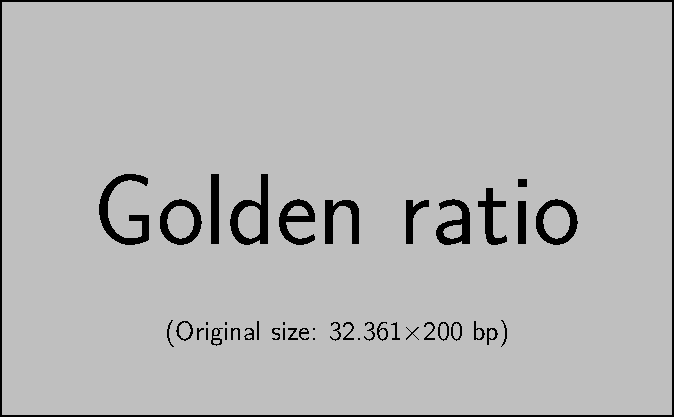
\includegraphics{placeholder_images/example-image-golden.pdf}
    \caption[Stacking of layers within a pouch cell]
    {Image showing the stacking of layers within a pouch cell. For the negative
        electrodes, there is a small overhang (\approx\SI{2}{mm}) at the
        edges with respect to the positive electrodes. This design choice
    helps to avoid plating of lithium at the edges.}
    \label{fig:anodeoverhangpouchcell}
\end{figure}

Thus,~\cref{eq:basiccapacitybalance} reduces to
\begin{equation}
    \frac{l_\text{neg}}{l_\text{pos}} = \frac{\varepsilon_\text{pos}}{\varepsilon_\text{neg}} = 1.22
\end{equation}
yielding $l_\text{neg} = \SI{72}{\micro\meter}$.

At first, it  may be surprising to  note that the values of  the particle radius
$R_\pj$ used in  both the \gls{p2d} and \gls{spm} remain  identical. However, it
is important  to note that  the \gls{p2d} equations  of the \gls{dfn}  model are
cast in  a normalised  form, \ie{}  already set  up to  account for  the overall
capacity of the  cell under consideration implicitly through usage  of a current
density  (per unit  area) for  its  simulation. Furthermore,  this explains  why
increasing the  number of  discretisation nodes does  not increase  the modelled
capacity, but  instead serves to improves  the simulation accuracy owing  to the
enhanced spatial resolution.

The  overall  active  surface  area  $A  =  n  A_\text{elec}$  is  the  combined
cross-sectional  area  of all  layers  ($n$  is  the number  of  electrochemical
(pos,sep,neg) triplets) stacked  into the pouch cell. In both  the \gls{p2d} and
\gls{spm}  models, this  parameter serves  to  scale the  external load  current
down  to  the current  density  experienced  by  each electrochemical  layer.  A
value  of  \approx\SI{30}{\ampere \per  \meter  \squared}  was reported  in  the
results section of  Subramanian~\etal{}~\cite{Subramanian2009}. When considering
a \SI{60}{\ampere\hour} pouch cell with \SI{10}{\milli\meter} exterior thickness
and  using  the  parameters  reported  in~\cite{Subramanian2009},  this  results
in  a cross-sectional  area of  \SI{2.053}{\meter\squared}\fxnote{to add:  refer
to  layer  optimisation  chapter   for  detailed  derivation}.  Considering  the
equalisation of capacity  loading, with the newly chosen thickness  value of the
negative  electrode, the  1C-rate  capacity  of the  cell  has  been revised  to
\SI{29.23}{\ampere\per\meter\squared}.

On  simulating  the \gls{p2d}  model  with  a  trickle bleeding  type  discharge
corresponding   to   a  current   of   C/500   and   logging  the   data   every
\SI{1}{\milli\second}, after reaching \SI{2.7}{\volt}\footnote{From manufacturer
    datasheets  for \protect{\gls{lco}}  chemistries,  this value  is considered  to
correspond to \SI{0}{\percent} \protect{\gls{soc}}.}, the remnant concentrations
in  the two  electrodes  were noted.  The  corresponding residual  stoichiometry
values  are reported  in~\cref{tbl:lcoSimParamsSPMp2d}  and  is consistent  with
typical values reported in literature for \gls{lco} chemistries.\fxnote{citation
needed here.}  This validation is  important, since below  certain stoichiometry
thresholds, the spinel/olivine  structure of the electrodes  can become unstable
and  collapse\fxnote{citation needed?}.

Since   the   cell   behaviour   is   considered   isothermal,   the   parameter
table     in~\cref{tbl:lcoSimParamsSPMp2d}     omits     activation     energies
for    the   various    diffusivities    and    conductivities   of    materials
(see~\cref{subsec:basicspmsimsetup}  for  further thermal  considerations).  For
this  reason,~\cref{tbl:lcoSimParamsSPMp2d}  does  not  include  other  material
properties such  as specific  heats, and  thermal conductivities.  No properties
of  the  current  collectors  appear  in  the  isothermal  model  equations  for
both  the \gls{p2d}  and  \gls{spm}  models and  hence  are  omitted. All  other
electrochemical  properties,   \viz{}  stoichiometries   at  \SI{100}{\percent},
maximum concentrations, diffusivities, reaction  rate coefficients and \gls{ocp}
of  the two  electrodes remain  invariant  between the  \gls{p2d} and  \gls{spm}
models.

\subsection{Simulation Setup}\label{subsec:basicspmsimsetup}

For  reproducibility of  results, it  is important  to discuss  the system-level
parameters influencing simulation setup.

The  lower cutoff  voltage of  the cell  is chosen  to be  \SI{2.5}{\volt}. This
is  deliberately  kept  lower  than  the voltage  corresponding  to  the  cell's
\SI{0}{\percent},  \ie{}  \SI{2.7}{\volt}.  If set  above  \SI{2.7}{\volt}  even
at  infinitesimally small  discharge  currents, the  cell  would cut-off  before
achieving complete discharge. Choosing a value lower than \SI{2.7}{V} means that
the cell gets a chance to recover its terminal voltage, despite spikes in highly
dynamic  load  currents  that  might  bring the  voltage  below  this  threshold
momentarily. If a low-enough value is  not chosen, a system-level shutdown shall
be  initiated  despite possessing  the  ability  to  continue to  operate  after
recovery  of terminal  voltage.  In  this case,  choosing  a  cutoff voltage  of
\SI{2.5}{\volt}  does  not  damage  the  cell  since  checks  are  in  place  to
monitor  the \gls{soc}  and  trigger cutoff  in the  event  of charge  depletion
(see~\cref{alg:ctstimespm,alg:disctimespm}).  Northrop~\etal~\cite{Northrop2011}
use this value, although no explanation is given for the choice.

The  upper  cutoff voltage  of  the  cell  is  chosen at  \SI{4.3}{\volt}  \ie{}
\approx\SI{100}{\milli  \volt}   higher  than   the  equilibrium   \gls{ocp}  at
\SI{100}{\percent} \gls{soc}. There are several  reasons for this smaller margin
at the upper end of the voltage spectrum
\begin{description}[leftmargin=!,labelwidth=\widthof{\bfseries low
    probabilities},itemsep=1ex]

\item[safety] li-ion  cells are less  tolerant to overcharging and  can pose
    fire hazards.

\item[degradation]  overcharging  li-ion  cells  can  lead  to  plating  and
    accelerate other degradation mechanisms.

\item[low  C-rates]  charging C-rates  are  typically  lower than  discharge
    C-rates.

\item[CCCV charging]  For on-board  chargers, taper charging  (such as  in a
    \gls{cccv} profile) is activated, which  ensures that charging current drops
    off  rapidly, leading  to a  lower overvoltage  towards the  upper \gls{soc}
    range.

\item[low probabilities] The only charging event when an electrified vehicle
    is in motion is during regenerative braking. The vehicular \gls{bms} manages
    the operating window such that the starting \gls{soc} is much lower than the
    overvoltage  that  could  be  caused due  to  braking.  Furthermore,  during
    operation, the net discharge events  occur more frequently than regenerative
    braking events.

\end{description}

For  both the  \gls{p2d} model  and the  \gls{spm} model,  the cell  temperature
is   kept   constant   at   its   initial   value   of   \SI{25}{\degreeCelsius}
(\SI{298.15}{\kelvin}). This implies that the  operation of the lithium ion cell
is assumed  to be isothermal.  While this  is not true  in general, it  is worth
noting that thermal gradients in  the through-thickness direction is negligible.
\fxnote{citation needed} Furthermore, for  the C-rates considered (<5C), typical
in a \gls{bev} application and  for short-duration transient loads studied, this
is a reasonable assumption. Detailed modelling of thermal dynamics is not within
the scope of this thesis, as the primary goal is to obtain a physics based model
incorporating  electrochemical  principles  amenable for  embedded  application.
Thus, thermal dependence of parameters through an Arrhenius-type relationship is
not  considered.    Future   work  could   include  performing   thermally  coupled
simulations, incorporating  thermally relevant  parameters and use  a simplified
heat generation expression,  \eg{} a lumped thermal model in  both the \gls{spm}
and \gls{p2d} and compare their performances.

To  understand  the parametrisation  of  initial  concentration, the  expression
for   electrolyte   conductivity   needs    to   be   examined.   As   discussed
in~\cref{subsec:spmp2dparametrisation}, the intrinsic conductivity of a specific
type  of  electrolyte  is  a  material   property  that  depends  on  the  local
concentration of \ch{Li^+} ions and  temperature. In the characterisation of the
electrolyte in Valøen and  Reimers~\cite{Valoen2005}, the polynomial expression
in~\cref{eq:kappavsCeandT} was obtained for the electrolyte conductivity.
\begin{multline}\label{eq:kappavsCeandT}
    \kappa_j(c_\text{e},T)(x,t) =  10^{-4} c_\text{e}(x,t) \bigl(-10.5 + \num{0.668e-3} c_\text{e}(x,t) + \num{0.494e-6}  c_\text{e}{(x,t)}^2\\
    + (0.074 - \num{1.78e-5}) c_\text{e}(x,t) - \num{8.86e-10} c_\text{e}{(x,t)}^2 \bigr)T(t)\\
	+ \left(\num{-6.96e-5} + \num{2.8e-8} c_\text{e}{(x,t)})T(t)^2\right)^2
\end{multline}

\begin{figure}[!htb]
    \centering
    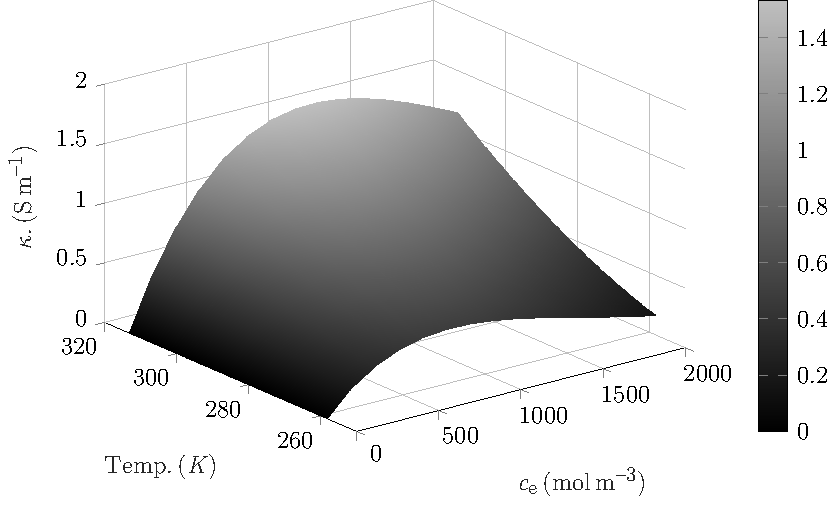
\includegraphics{4/figures/m2t_kappa_ce_T.pdf}
    \caption[Surface plot of electrolyte conductivity]
    {Electrolyte conductivity as a function of cell temperature and initial
        concentration. The variation of conductivity versus these factors is a
    smooth function.}
    \label{fig:kappavsCeandT}
\end{figure}

\Cref{fig:kappavsCeandT} shows  a surface  plot of the  electrolyte conductivity
as  a function  of  initial concentration  $c_\text{e,0}$  and cell  temperature
$T_\text{cell}$.\fxnote{comment on how the variation in the direction of temp is
less significant to that around conc} In particular,
\begin{enumerate}%[label=\emph{\alph*})]
    \item At  equilibrium  initial condition ($t=0$), $c_\text{e}$ is uniform over the axial space $x$ and
    \item only isothermal cell behaviour is considered, \ie{} $T(t) = T_\text{cell}$.
\end{enumerate}
Hence,~\cref{eq:kappavsCeandT} reduces to
\begin{multline}\label{eq:kappavsCeinitandTcell}
    \kappa_j =  10^{-4} c_\text{e,0} \bigl(-10.5 + \num{0.668e-3} c_\text{e,0} + \num{0.494e-6}  c_\text{e,0}^2\\
        + (0.074 - \num{1.78e-5}) c_\text{e,0} - \num{8.86e-10}
    c_\text{e,0}^2 \bigr)T_\text{cell}\\
	+ \left(\num{-6.96e-5} + \num{2.8e-8} c_\text{e,0})T_\text{cell}^2\right)^2
\end{multline}
As   inferred   from~\cref{fig:kappavsCeandT},  the   electrolyte   conductivity
$\kappa$   is   a  smooth   function   of   $c_\text{e}$  and   $T_\text{cell}$.
Thus~\cref{eq:kappavsCeinitandTcell}  can be  effectively  visualised through  a
parametric plot of $\kappa$ vs  $c_\text{e}$ with $T_\text{cell}$ as the varying
parameter as seen in~\cref{fig:kappavsce}.

\begin{figure}[!htb]
    \centering
    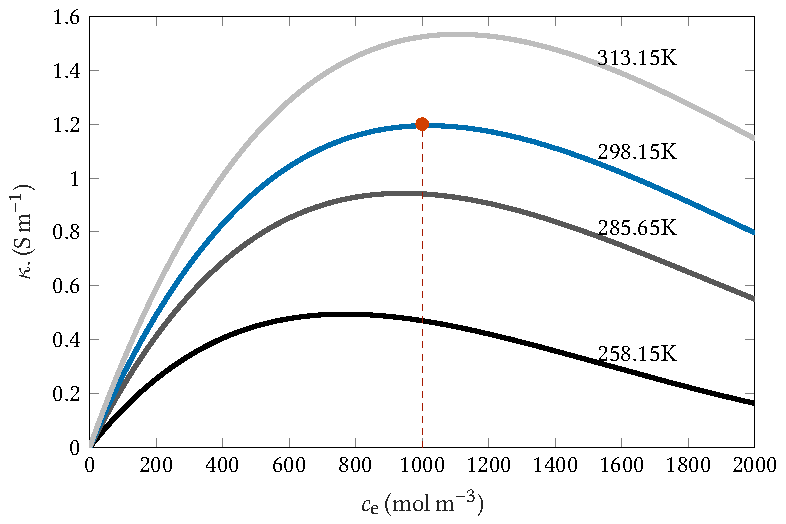
\includegraphics{4/figures/m2t_kappa_ce_parametric_T.pdf}
    \caption[]
    {Electrolyte conductivity versus equilibrium concentration at various cell
        temperatures. At ${T_\text{cell} = \SI{298.15}{\kelvin}}$, the maximum
        value of electrolyte conductivity corresponds to a salt concentration of
    \SI{1000}{\mol\per\meter\cubed}.}
    \label{fig:kappavsce}
\end{figure}

From~\cref{fig:kappavsce},       it        is       evident        that       at
$T_\text{cell}=\SI{298.15}{\kelvin}$,   the   maximum   value   of   electrolyte
conductivity is attained at  $c_\text{e} = \SI{1000}{\mole\per\meter\cubed}$. It
is advantageous  to operate  the cell  around this salt  concentration so  as to
minimise  the  cell's  overall  resistance.  Hence,  the  initial  concentration
$c_\text{e,0}$ is  chosen to  be \SI{1000}{\mole\per\meter\cubed}. It  should be
noted that while  the electrolyte concentration in the  \gls{p2d} model exhibits
both spatial  and temporal  variations during the  simulation, in  the \gls{spm}
model, it remains constant throughout.

The      reduction      in      parametrisation      requirements      discussed
in~\cref{subsec:spmp2dparametrisation}    is   only    one   of    the   factors
contributing  to   the  simplicity   and  ease   of  simulation.   As  discussed
in~\cref{subsec:basicspmgeometry},   an   important  computational   requirement
that   is  present   in   the  \gls{p2d}   model,   but  completely   eliminated
from  the   \gls{spm}  is  the   requirement  of  discretisation.   As  reported
in~\cref{tbl:lcoSimParamsSPMp2d},  with  15 nodes  per  region  along the  axial
direction  and  with 10  shells  per  electrode  in  the radial  direction,  the
\gls{p2d}  model under  simulation  achieves mesh  independence  to a  tolerance
of  \approx   \SI{2}{\percent}  for  the   range  of  C-rates   considered.  For
higher  C-rates,  coupling  a  thermal   model  is  of  higher  importance  than
incorporating further meshing refinements. The discretisation-related parameters
are  specific to  the  \gls{p2d}  model and  is  hence, highlighted  accordingly
in~\cref{tbl:lcoSimParamsSPMp2d}.

With  the cell  parametrisation discussed  and the  simulation setup  presented,
the  simulation   results  are  fully   reproducible  and  are   presented  next
in~\cref{subsec:simresultsbasicspm}.

\subsection{Simulation Results}\label{subsec:simresultsbasicspm}

\subsubsection*{Capacity Characterisation}\label{subsubsec:capcharspmp2d}

First,  it  must be  established  that  incorporating the  parameters  presented
in~\cref{tbl:lcoSimParamsSPMp2d} into the \gls{spm} model equations results in a
cell with  \emph{identical} capacity as the  \gls{dfn} model. This is  to ensure
the  validity  of  comparisons  in  further simulations.  Using  the  values  of
per-layer  C-rate as  discussed  in~\cref{subsec:spmp2dparametrisation} and  the
overall active  surface area from~\cref{tbl:lcoSimParamsSPMp2d}, the  cell under
simulation has a capacity of \SI{60}{\amphour}.

For experimental capacity characterisation of cells, the standard practice is to
apply a very small discharge  current beginning at \SI{100}{\percent} \gls{soc},
logging the charge passed using a  high-precision coulomb counter until the cell
hits the voltage corresponding to \SI{0}{\percent} \gls{soc} as specified in the
manufacturer datasheet. In  order to decouple the effect of  the cell's dynamics
from its  capacity, it is  required to  apply an infinitesimal  bleeding current
(tending towards, but should not reach \SI{0}{\ampere}).

Current sensors in battery cycler equipment use high-precision (typically 15--18
bit) \glspl{adc}  and are  able to  offer high  \glspl{snr} except  at ultra-low
currents. The main difficulty with using very low C-rates is that it drastically
slows down the  characterisation procedure. Using a discharge  current of C/100,
\ie{}  \SI{0.6}{\ampere} in  this case,  results in  a characterisation  time of
\SI{100}{\hour} or \approx $4\sfrac{1}{4}$  days (excluding soak-times and other
set-up related  activities). Furthermore, for accurate  coloumb-counting, a high
data logging  rate is needed,  resulting in  large file sizes  and corresponding
difficulties in post-processing them.  Considering moderate buffer-sizes used in
data logging modules of typical  cell-cycler software (shared between channels),
and  to  avoid  excessively  large wait-times  for  characterisation,  discharge
currents of C/20--C/25 are usually deemed sufficient.

An analogous  procedure is  carried out in  numerically characterising  the cell
capacities through computer  simulation. However, this approach is  not bound by
real-world issues such as low  \glspl{snr} or long characterisation times. Using
64-bit IEEE  floating point arithmetic,  numbers as low  as $\mathcal{10^{-16}}$
can be safely computed, nullifying any  \gls{snr} issues. The simulation time of
both the  \gls{p2d} and  \gls{spm} models  are much  faster than  real-time. The
only  persistent issue  here  is that  of memory  and  storage requirements  due
to  high-rate  data-logging for  accurate  coloumb  counting. Nevertheless,  the
data-logging reliability of a dedicated computer workstation far exceeds that of
real-time cell cyclers and facilitates the desired numerical characterisation of
cell capacity.

\begin{figure}[!htb]
    \centering
    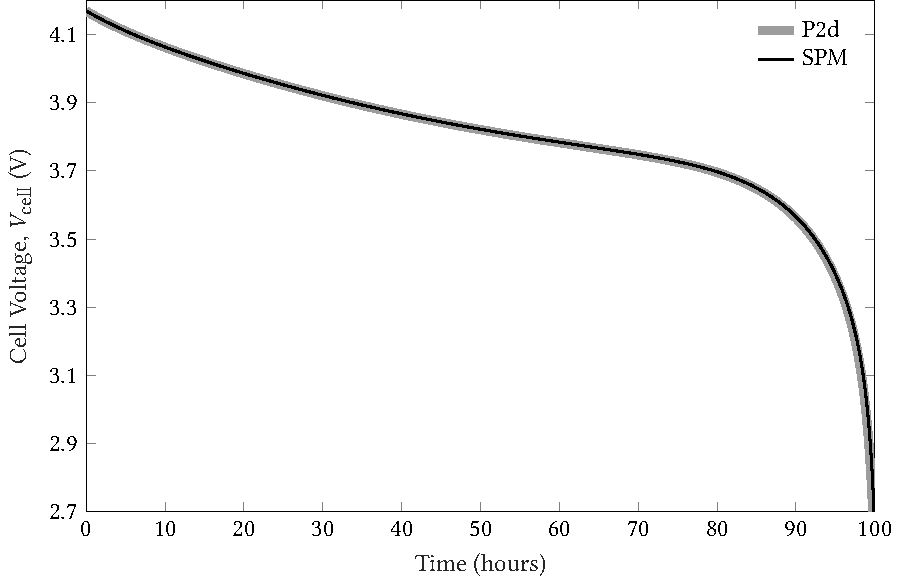
\includegraphics{4/figures/capacity_match_spm_p2d.pdf}
    \caption[Capacity characterisation of \glsfmtshort{spm} and \glsfmtshort{p2d}
    models]{Capacity characterisation of the cell by numerically simulating the
        \gls{p2d} and \gls{spm} models with an ultra-low discharge current of
        C/100, \ie{} \SI{0.6}{A}. The time-domain voltage response of both
        models overlap. The \gls{p2d} and \gls{spm} models both achieve their
        charge depletion point \ie{} \SI{0}{\percent} \gls{soc} after
        \SI{100}{\hour} confirming that the modelled capacities match. Key data
    for this characterisation run is shown in~\cref{tbl:charSimspmp2d}.}
    \label{fig:capcharspmp2d}
\end{figure}

In order to validate  that the choice of model parameters  result in an intended
capacity  of  \SI{60}{\amphour},  a  characterisation  simulation  beginning  at
\SI{100}{\percent}  \gls{soc}  with  a discharge  current  of  \SI{0.6}{\ampere}
was   performed\footnote{All   simulations   were    performed   on   a   64-bit
Hewlett-Packard  Z840  workstation  with a  16-core  \text{Intel}\textregistered
Xeon\textregistered E5-2640 v3 (Haswell) processor at \SI{2.60}{\giga\hertz} and
\SI{128}{\giga\byte} DDR4 RAM at 1866 MT/sec.}.  If the assumed cell capacity is
indeed consistent with  the model parameters, then this corresponds  to a C-rate
of  \sfrac{1}{100}, and  the  \gls{p2d}  and \gls{spm}  should  run for  exactly
\SI{100}{\hour} before charge depletion  cut-off. For accurate coulomb counting,
data logging interval is set to \SI{50}{\milli\second}. \Cref{fig:capcharspmp2d}
shows the voltage  response of the \gls{spm} and \gls{p2d}  models obtained. The
voltage  responses  of  both  the  models  overlap,  and  they  both  achieve  a
run-time  of \approx\SI{100}{\hour}.  This capacity  characterisation simulation
represents the  first visualisation of  results produced by the  \gls{spm} model
equations  discussed  in~\cref{subsec:basicspmgoverningeqns} and  its  numerical
implementation from~\cref{sec:numericalimplementation}. \Cref{tbl:charSimspmp2d}
summarises the key data from the capacity characterisation simulation.

% -*- root: ../main.tex -*-
%!TEX root = ../main.tex
% this file is called up by main.tex
% content in this file will be fed into the main document

\begin{table}[!htb]
    \centering
    \caption[Simulation data --- capacity characterisation of \glsfmtshort{p2d} and \glsfmtshort{spm} models]{Simulation data --- capacity characterisation of \glsfmtshort{p2d} and \glsfmtshort{spm} models. The \glsfmtshort{p2d} model is taken as the benchmark. Hence, modelling error is defined as \protect{$\varepsilon = V_\text{cell,p2d} - V_\text{cell,spm}$}.}
    \label{tbl:charSimspmp2d}
    \begin{tabular}{@{} l r r @{}}
        \toprule
        Parameter                                                       & Value  & Units              \\
        \midrule
        Data-logging interval                                           & 50.00  & \si{\milli\second} \\
        Total RAM used                                                  & 603.90 & \si{\mega\byte}    \\
        \glsfmtshort{p2d} run-time                                      & 99.94  & \si{\hour}         \\
        \glsfmtshort{spm} run-time                                      & 99.90  & \si{\hour}         \\
        \glsfmtshort{p2d} discharge capacity                            & 59.96  & \si{\amphour}      \\
        \glsfmtshort{spm} discharge capacity                            & 59.94  & \si{\amphour}      \\
        Max error, $\varepsilon_\text{max}$                             & -94.30 & \si{\milli\volt}   \\
        \glsfmtshort{rms} error, $\varepsilon_\text{\glsfmtshort{rms}}$ & 8.20   & \si{\milli\volt}   \\
        \glsfmtshort{mae} error, $\varepsilon_\text{\glsfmtshort{mae}}$ & 3.20   & \si{\milli\volt}   \\
        \bottomrule
    \end{tabular}
\end{table}

% explain the table next.

Thus, a common baseline is established  by confirming that the two models indeed
simulate a cell with the desired capacity.

% electrolyte resistance
